% !TEX root = thesis.tex

\section{El polinomi de Jones}\label{sec:El polinomi de Jones}

El descobriment del \textit{polinomi de Jones} per part de Vaughan Jones l'any 1984 [\cite{jonesoriginal}] dona una manera d'associar a cada nus o link un polinomi de Laurent amb coeficients enters. Aquesta correspondència es fa mitjançant un diagrama de link qualsevol. La teoria de Jones es fonamenta en el fet que si fem un moviment RI, RII o RIII al diagrama del link, aquest polinomi no canvia i doncs és un invariant sota moviments de Reidemeister. El polinomi per un link és doncs independentment del diagrama d'aquest. De manera que si podem veure que dos diagrames de links no tenen el mateix polinomi, llavors segur que aquests son diferents.\\

\subsection{Construcció del polinomi de Jones}

La manera més simple per definir-lo és mitjançant un altre tipus de polinomi; el \textit{polinomi de Kauffman} descobert per Louis Kauffman.\\

\begin{definition}
	El \underline{polinomi de Kauffman} de $L$, $\langle L\rangle$ és un polinomi de Laurent amb coeficients enters i indeterminada $A$ que podem associar a tot diagrama d'un link a $S^2$ de la següent manera:
	\begin{enumerate}
		\item\label{item:i} $\left\langle\KPA\right\rangle=1$
		\item\label{item:ii} $\left\langle L \cup \KPA\right\rangle=(-A^{-2}-A^{2})\langle L\rangle$
		\item\label{item:iii} $\left\langle\KPB\right\rangle=
		A\left\langle\KPC\right\rangle + A^{-1} \left\langle \KPD \right\rangle$
	\end{enumerate}
\end{definition}

En aquesta definició, $$\KPA$$ representa el diagrama del nus trivial i $$L \cup \KPA$$ és un diagrama de $L$ juntament amb una corba tancada extra que no conté cap creuament ni amb ella mateixa ni amb $L$. A \textit{\ref{item:iii}} la fórmula relaciona tres diagrames que son el mateix excepte al voltant d'un creuament on es diferencien pels moviments locals indicats. A partir d'aquesta definició és fàcil veure les següents propietats.

\begin{enumerate}
	\item\label{item:1} $\left\langle\KPA\stackrel{c}{\dots}\KPA\right\rangle=(-A^{-2}-A^{2})^{c-1}$
	\item\label{item:2} $\left\langle L\right\rangle=\left\langle rL\right\rangle$
\end{enumerate}

Per demostrar \ref{item:1} només cal fer inducció sobre $c$ utilitzant la propietat \textit{\ref{item:iii}} del polinomi de Kauffman. Per \ref{item:2} és evident ja que el polinomi de Kauffman no té en compte d'orientació del nus alhora de calcular-lo.\\

Investiguem ara el comportament del polinomi respecte els moviments de Reidemeister.

\begin{lemma}\label{lem:RI}
	Si a $K$ hi apliquem un moviment RI el seu polinomi de Kauffman es veu multiplicat per un factor de $-A^{-3}$.
\end{lemma}

\begin{proof}
	Utilitzant \textit{\ref{item:iii}} i \textit{\ref{item:ii}} en aquest mateix ordre.
\end{proof}

Notem a més que si a \textit{\ref{item:iii}} fessim un moviment local canviant-lo a $$\KPI$$ llavors el polinomi de Kauffman corresponent seria el mateix que l'original intercanviant $A$ per $A^{-1}$.\\

La Figura \ref{fig:calculpolinomidekauffman} mostra de forma iterativa el càlcul d'aquest polinomi. Així doncs trobem que $$\left\langle 3_1\right\rangle=A^{-7}-A^{-3}-A^{5}$$ Un exercici similar demostra que $$\left\langle \overline{3_1}\right\rangle=A^{7}-A^{3}-A^{-5}$$

Elaborant el que acabem de veure, si $\overline{K}$ és el nus emmirallat de $K$, llavors $\left\langle\overline{K}\right\rangle=\overline{\left\langle K\right\rangle}$, on $\overline{\left\langle K\right\rangle}$ denota el canvi esmentat anteriorment. Observem com $\left\langle\overline{3_1}\right\rangle$ també verifica el que acabem de veure.

\begin{figure}
	\centering
	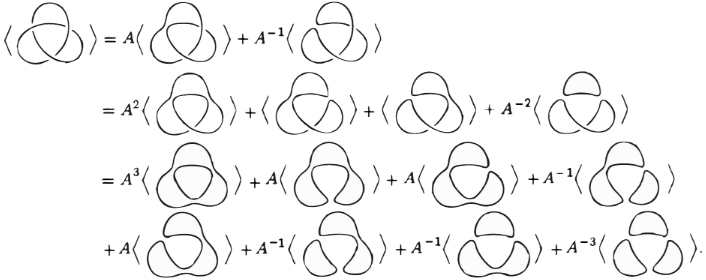
\includegraphics[width=\linewidth]{img/polinomidekauffman.png}
	\caption{Exemple del polinomi de Kauffman de $3_1$.}\label{fig:calculpolinomidekauffman}
\end{figure}

\begin{lemma}\label{lem:RIIiRIII}
	El polinomi de Kauffman és invariant per moviments RII i RIII.
\end{lemma}

\begin{proof}
	Per RII cal aplicar \textit{\ref{item:iii}} dues vegades seguides sabent que $\left\langle\overline{K}\right\rangle=\overline{\left\langle K\right\rangle}$ i aplicar-ho en un dels dos creuaments. Per RIII cal fer exactament el mateix.
\end{proof}

\begin{definition}\label{def:torçament}
	Definim el \underline{torçament} $w(L)$ del diagrama d'un link orientat qualsevol com la suma dels signes dels seus creuaments, on cada un d'aquests pren el valor $+1$ o $-1$ com s'indica a la Figura \ref{fig:signe}
\end{definition}

\begin{figure}
	\centering
	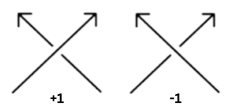
\includegraphics[width=0.6\linewidth]{img/signe.png}
	\caption{Signe d'un creuament per la regla de la ma dreta.}\label{fig:signe}
\end{figure}

Notem que la Definició \ref{def:torçament} utilitza la orientació del link. Un simple exercici demostra que aquest és invariant sota moviments RII i RIII i aquest canvia per $+1$ o $-1$ sota moviments RI. La Figura \ref{fig:calculdelsigne} mostra dos exemples sobre el càlcul del torçament d'un nus.\\

\begin{figure}
	\centering
	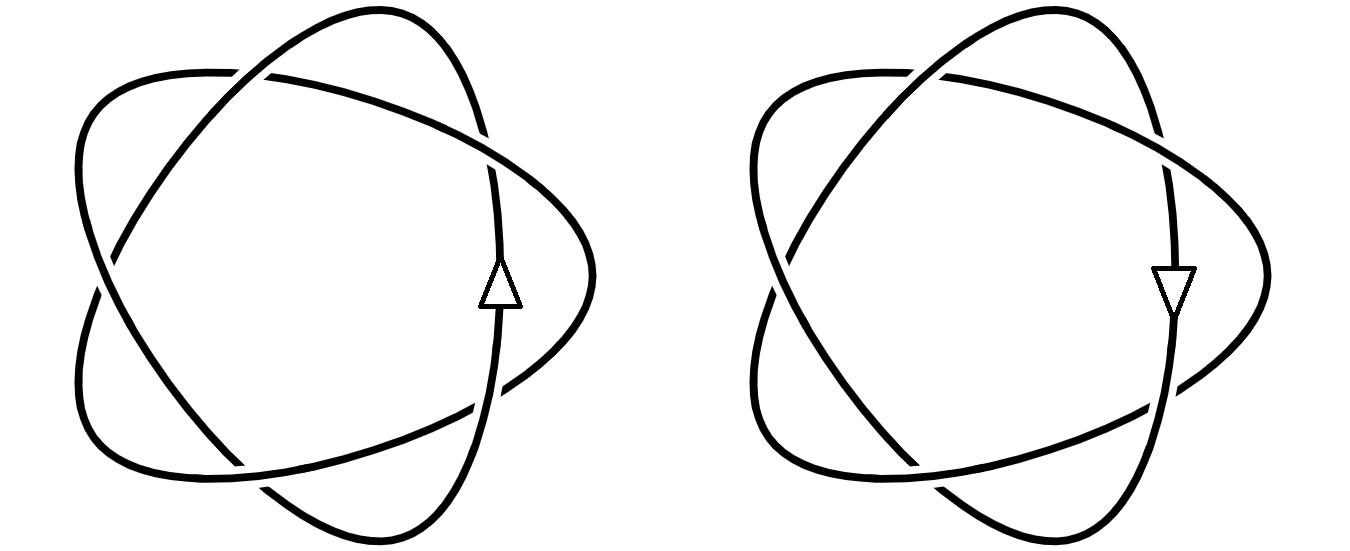
\includegraphics[width=0.9\linewidth]{img/torçament.png}
	\caption{A l'esquerra el nus $5_1$ que té torçament -5, a la dreta $r5_1$ que té torçament també -5.}\label{fig:calculdelsigne}
\end{figure}

El torçament d'un link orientat juntament amb el polinomi de Kauffman d'un diagrama de link sense tenir en compte l'orientació son tots dos invariants sota moviments RII i RIII a més, aquests es comporten d'una manera previsible sota moviments RI. Això duu al següent resultat:

\begin{theorem}
	Sigui $diag(L)$ un diagrama d'un link orientat $L$. Llavors, $$(-A)^{-3w(L)}\left\langle L\right\rangle$$ és un invariant del link orientat $L$.
\end{theorem}

\begin{proof}
	Conseqüència directa del Lema \ref{lem:RIIiRIII}, el Lema \ref{lem:RI} i l'observació sobre el torçament sota moviments RI anterior.
\end{proof}

\begin{definition}\label{def:polinomidejones}
	El \underline{polinomi de Jones} $V(L)$ d'un link orientat $L$ és el polinomi de Laurent en $t^{1/2}$ i coeficients enters, i.e. $\mathbb{Z}[t^{1/2},t^{-1/2}]$, definit per $$V(L)=\left((-A)^{-3w(L)}\left\langle L\right\rangle\right)_{t^{1/2}=A^{-2}}$$ on $\left\langle L\right\rangle$ és el polinomi de Kauffman i $w(L)$ és el torçament definits anteriorment.
\end{definition}

Aquí, $t^{1/2}$ és una indeterminada el quadrat de la qual és $t$. De fet, es pot veure per inducció que només els links amb un nombre senar de components, incloent els nusos tenen polinomi amb potències enteres de $t$. El polinomi de Jones està ben definit i a més, $V(\ovoid)=1$. De fet, no es coneix cap altre exemple de nus $L$ pel qual $V(L)=1$; trobar un nus tal o demostrar que no existeix es considera un problema important. La Figura \ref{fig:polinomidejones} mostra una taula amb els polinomis de Jones de fins a 7 creuaments utilitzant l'algorisme descrit anteriorment.\\

\begin{figure}
	\centering
	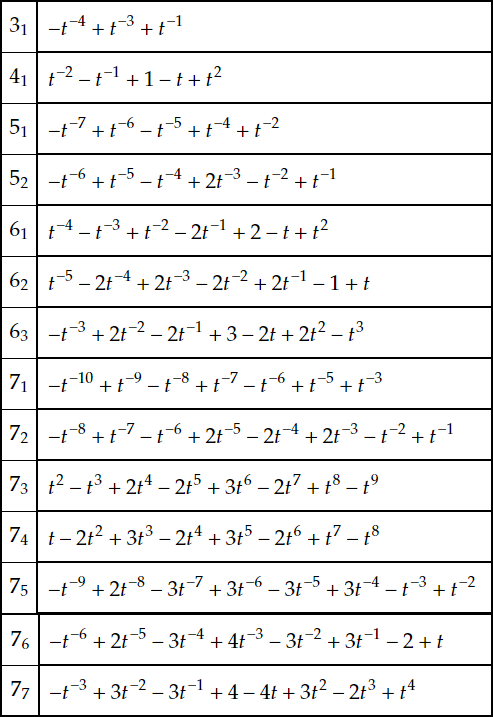
\includegraphics[width=\linewidth]{img/jonestaula.png}
	\caption{Taula dels polinomis de Jones. Una simple observació permet veure que tots aquests son diferents entre si.}\label{fig:polinomidejones}
\end{figure}

Clarament, si l'orientació de cada component del link canvia, llavors el signe en cada creuament es manté constant. Així doncs, el polinomi de Jones d'un nus no depèn de l'orientació escollida. Dit d'una altra manera, el polinomi de Jones no distingeix un nus $K$ del seu invers $rK$. Pel que fa la quiralitat, el polinomi de Jones tampoc té perquè distingir-los tot i que hi ha certes circumstàncies en que si, i doncs es comporta millor en distingir nusos amb aquesta darrera propietat. Elaborant en aquest últim comentari, utilitzant la Definició \ref{def:polinomidejones} no és massa difícil veure que $$V(3_1)=-t^{-4}+t^{-3}+t^{-1}$$ i $$V(\overline{3_1})=t+t^3-t^4$$ així doncs sabem que $3_1\neq\overline{3_1}$ i doncs no existeix cap isotopia ambient que passi d'un a l'altre.\\

\begin{definition}\label{def:nombredenllaç}
	Sigui $L$ un link orientat amb dues components $L_1$ i $L_2$. El \underline{nombre de nuament} $lk(L_1,L_2)$ de $L_1$ i $L_2$ és la meitat de la suma dels signes del seu diagrama els creuaments dels quals son sobrepassos.
\end{definition}

La Figura \ref{fig:nombredenuament} dona un exemple d'aquest càlcul.\\

\begin{figure}
	\centering
	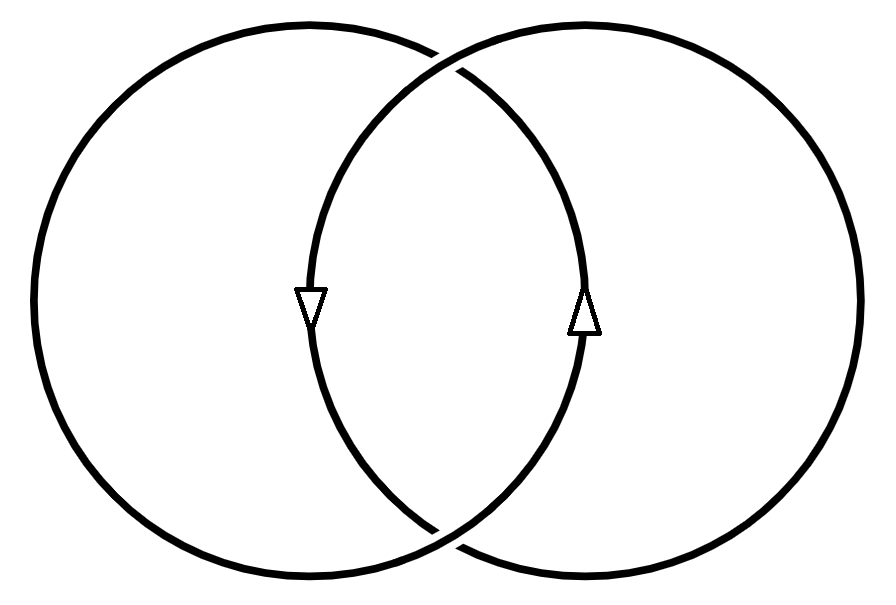
\includegraphics[width=0.6\linewidth]{img/nombredenuament.png}
	\caption{Càlcul del nombre de nuament del link de Hopf. Aquest té nuament -1.}\label{fig:nombredenuament}
\end{figure}

És fàcil veure que si a un link orientat $L$ se li canvia l'orientació de només una component $K$ donant lloc a $L'$, llavors $$V(L')=t^{-3lk(K,L-K)}V(L)$$ d'aquesta manera el polinomi de Jones depèn de l'orientació d'una manera molt elemental.\\

El polinomi de Jones es caracteritza mitjançant el següent resultat que és una conseqüència directa de la Definició \ref{def:polinomidejones}.\\

\begin{proposition}\label{prop:jones}
	El polinomi de Jones és una funció $$V:\{\text{Link orientat a }S^3\}\rightarrow \mathbb{Z}[t^{-1^2},t^{1/2}]$$ de manera que
	\begin{enumerate}
		\item $V(\ovoid)=1$
		\item\label{item:skeinrelation} Sempre que tres links orientats $L_{+}$, $L_{-}$ i $L_{0}$ siguin el mateix excepte al voltant d'un punt, llavors $$t^{-1}V(L_{+})-tV(L_{-})+(t^{-1/2}-t^{1/2})V(L_{0})=0$$
	\end{enumerate}
\end{proposition}

on $L_{+}, L_{-}, L_{0}$ son links havent fet un moviment local a un dels creuaments.

\begin{proof}
	Sabem
	\begin{align}
		\label{eq:eq1}\left\langle\KPB\right\rangle=
		A\left\langle\KPC\right\rangle + A^{-1} \left\langle \KPD \right\rangle\\
		\label{eq:eq2}\left\langle\KPI\right\rangle=
		A^{-1}\left\langle\KPC\right\rangle + A \left\langle \KPD \right\rangle
	\end{align}
	Multiplicant \ref{eq:eq1} per $A$ i \ref{eq:eq2} per $A^{-1}$ i restat les dues equacions obtenim $$A\left\langle\KPB\right\rangle-A^{-1}\left\langle\KPI\right\rangle=(A^2-A^{-2})\left\langle\KPC\right\rangle$$
	D'aquesta manera, per links orientats amb diagrames com els mostrats, utilitzant el fet que $w(L_{+})-1=w(L_{0})=w(L_{-})+1$ tenim $$-A^4V(L_{+})+A^{-4}V(L_{-})=(A^{2}-A^{-2})V(L_{0})$$ Fent la substitució $t^{1/2}=A^{-2}$ dona el resultat buscat.
\end{proof}

Deduïm automàticament de la Proposició \ref{prop:jones} que si $L'$ és un link creat a partir de $L$ afegint un component trivial de més, llavors el seu polinomi de Jones ve donat per $V(L')=(-t^{-1/2}-t^{1/2})V(L)$. La Proposició \ref{prop:jones} anterior també permet el càlcul de qualsevol link orientat. Això és conseqüència directa del fet que tot link pot ser deformat fins a assolir el link trivial de $c$ components, el polinomi de Jones del qual és $(-t^{-1/2}-t^{1/2})^{c-1}$ a partir de fer moviments locals el un diagrama d'aquest.\\

De la mateixa manera que el gènere d'un nus, vist a la Secció \ref{sec:generescomainvariant} obtenim un resultat similar.\\

\begin{proposition}
	El polinomi de Jones de la suma de dos nusos $K$ i $K'$ és el producte dels seus polinomis de Jones, i.e. $$V(K+K')=V(K)V(K')$$
\end{proposition}

\begin{proof}
	Considerant la suma del dos nusos $K+K'$ i operant mitjançant la relació \ref{item:skeinrelation} en només un dels dos nusos trobem el seu polinomi de Jones, repetint el procés amb l'altra nus arribem al nus trivial.
\end{proof}



Per acabar la secció, cal remarcar que la teoria d'invariants és una teoria que preten desenvolupar diferents eines per tal de poder dur a terme la tasca de distingir els diferents nusos. Per aquest motiu, no hi ha invariants millors ni pitjors, sinó que cadacun d'ells ajuda en aquesta tasca i mentre possiblement un invariant no permeti distingir entre dos nusos, possiblement un altra si. També, volia remarcar que dins la teoria de nusos existeix una gran quantitat d'invariants que no s'han pogut discutir en aquest treball. Alguns d'ells son, la p-Colorabilitat, el Determinant, el polinomi d'Alexander, el polinomi de Conway, el Grup Fonamental o el polinomi de HOMFLY-PT. Aquest últim consisteix en una generalització del polinomi de Jones i el d'Alexander alhora, de manera que conté la informació de tots dos polinomis. Un exemple de nus amb els mateixos polinomis de Jones, Alexander i HOMFLY-PT és el famós nus de Conway i el de Kinoshita-Terasaka, $11n34$ i $11n42$ respectivament en la notació de Thistlethwaite. Aquests dos nusos es distingeixen perquè tenen diferent gènere, i grup fonamental. No obstant, presenten els mateixos polinomis discutits anteriorment. El mètode per construïr nusos d'aquesta mena és mitjançant un moviment introduït per Conway anomenat \textit{mutació}. La Figura \ref{fig:mutacio} mostra aquests dos nusos. Cal destacar que la teoria de nusos no té invariants complets, és a dir, que no existeix cap eina que permeti una classificació completa dels nusos i per tant, sempre existirà nusos diferents que cap de les eines desenvolupades pugui distingir. No obstant, hi ha certes classes de nusos pels quals el polinomi de HOMFLY n'és un invariant complet.

\begin{figure}
	\centering
	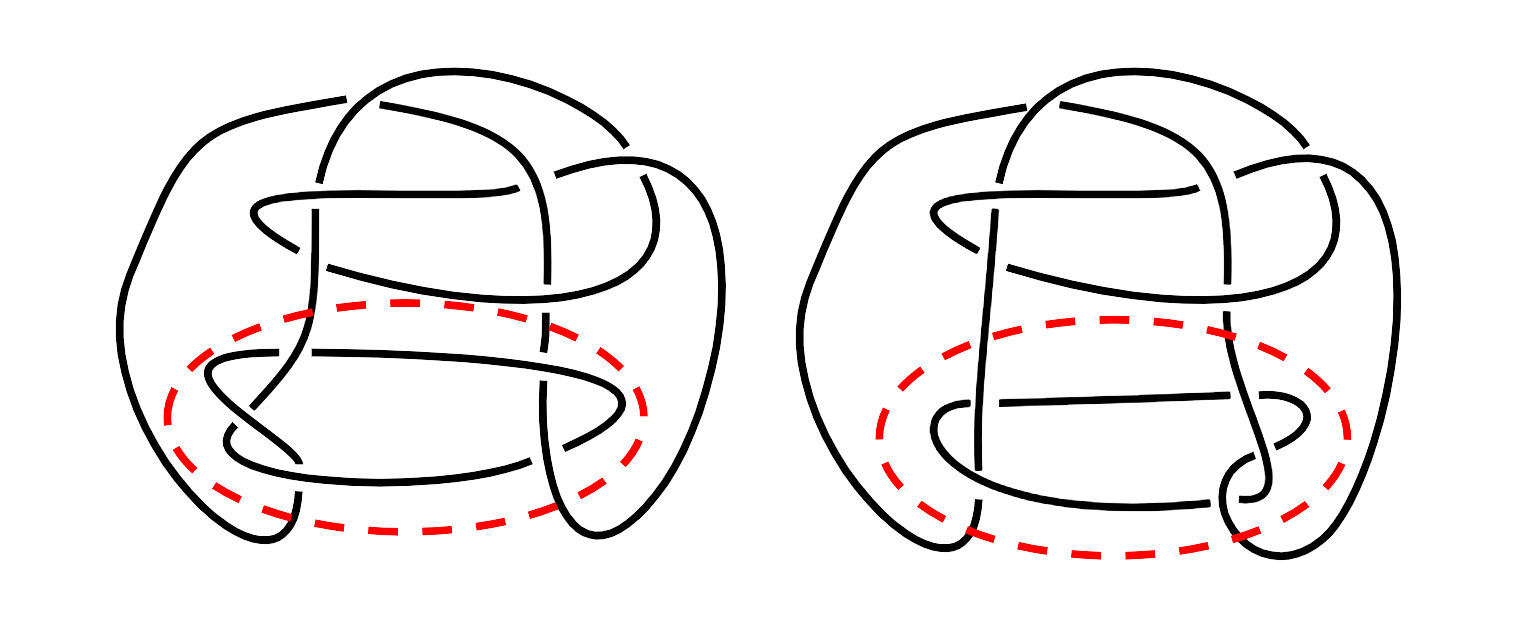
\includegraphics[width=\linewidth]{img/mutació.png}
	\caption{Exemple de mutació. D'esquerra a dreta: Nus de Kinoshita-Terasaka; $11n42$ i nus de Conway; $11n34$.}\label{fig:mutacio}
\end{figure}